\section{Patrycja Potoczek}


\subsection{Okrąg opisany na czworokącie}

Na czworokącie można opisać okrąg wtedy i tylko wtedy,
gdy sumy miar jego przeciwległych kątów wewnętrznych są
równe 180°
\[ \alpha + \gamma = \beta + \delta = 180^\circ \]

 \begin{figure}[htbp]
     \centering
     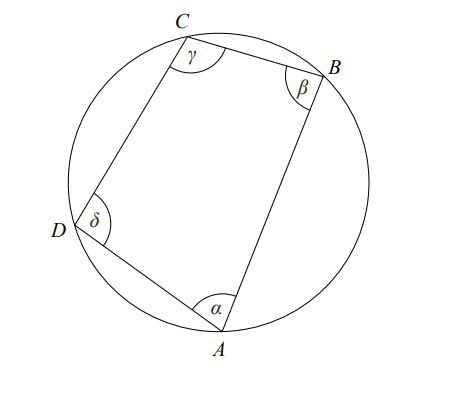
\includegraphics[width=0.6\textwidth]{pictures/okrag_na_czworokacie.jpg}
     \caption{\label{fig:okrag_na_czworokacie}Okrąg opisany na czworokącie}
 \end{figure}


\begin{table}[h]
\centering
\begin{tabular}{||c c c||} 
 \hline
 A & B & Y \\ [0.5ex] 
 \hline\hline
 0 & 0 & 0 \\ 
 \hline
 0 & 1 & 0 \\
 \hline
 1 & 0 & 0 \\
 \hline
 1 & 1 & 1 \\
 \hline
\end{tabular}
\label{tab:tabela5}
\caption{Tabela prawdy dla bramki logicznej AND}
\end{table}

\subsection{Lista numerowana i nienumerowana}

\begin{enumerate}
\item One theory is that the dollar sign comes from the Pillars of Hercules, as the Ancient Greeks
used to call the two rocks at the entrance to the Straits of Gibraltar. 
\item When King Ferdinand II of Aragon claimed the Straits of Gibraltar in 1492, he ordered the production of coins showing the Pillars of Hercules wrapped in a banner. 
\end{enumerate}
\begin{itemize}
\item When the Spanish colonized America, the coins travelled with them and so the Pillars of Hercules became a symbol of the New World. 
\item In the 18th and 19th centuries they also appeared on the Spanish dollar, known as the peso. This showed two columns with a ribbon wrapped around them in an S shape.
\item The similarity to the American dollar sign seems obvious. 
\end{itemize}


\subsection{Pierogi ruskie}

\textbf{Pierogi ruskie} – popularny wśród Polaków w Polsce i na Rusi rodzaj pierogów, których nazwa wywodzi się od Rusi Czerwonej (Galicja Wschodnia). \underline{Nie należy} jej mylić, jak to często jest robione, z Rosją, gdzie ten typ pierogów nie jest znany. \par
Dawniej bardzo popularne wśród Polaków mieszkających na terenach Rusi (województwa ruskiego Korony Królestwa Polskiego, następnie w Rzeczypospolitej). \emph{Na Ukrainie pierogi te bywają zwane „polskimi”}.


\subsection{Odniesienie}
Odniesienie do twierdzenia matematycznego - Figure \ref{fig:okrag_na_czworokacie}